\documentclass{article}
\usepackage{graphicx} % Required for inserting images
\usepackage{amsmath}
\usepackage{matlab-prettifier}
\usepackage{gensymb}
\usepackage[a4paper, margin=1in]{geometry} % Adjust margin here
\usepackage{chngcntr}
\usepackage{svg}

\counterwithin{table}{section}
\counterwithin{figure}{section}
\counterwithin{equation}{section}
\setlength{\parskip}{5pt}     % Space between paragraphs
\setlength{\parindent}{0pt}  % Indent at the start of each paragraph

\title{Throttle Modeling}
\author{Avionics \& Control Systems \\ Texas A\&M University Rocket Engine Design}
\date{April 24 2025}

\begin{document}

\maketitle
\tableofcontents
\newpage
\section{Introduction}

The first goal in throttle modeling is to acquire a mathematical relationship between the throttle position and the engine thrust. There are two ways to approach this. One is through a rigorous high-fidelity model of the engine, and the other is through test data.

The approach discussed in this document will follow system identification methodology with test data, however, both methods ultimately end up designing the throttle control algorithm through a simulation of the mathematical engine/throttle model. 

\section{Background}
Some background knowledge is desired to understand the motivation behind the throttling test process and design:

\begin{enumerate}
    \item Differential Equations
    \item Laplace Transforms
    \item Classical Control Theory
    \item Discrete-Time Control Systems
    \item Fourier Transforms
    \item System Identification
\end{enumerate}

The following sections are to bridge gaps in knowledge and bring the reader up to speed on the theory being used.

\subsection{Transfer Functions}
For a simple example, lets consider a spring-mass-damper system in Figure 1.1. The linear equation of motion for a spring-mass-damper is the differential equation Equation 1.1. 

\begin{figure}[h]
    \centering
    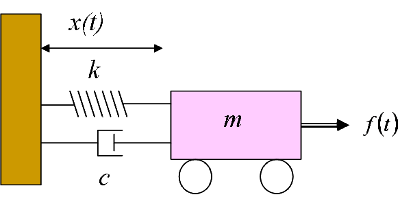
\includegraphics[width=0.5\linewidth]{figures/spring_mass_damper.png}
    \caption{Spring-Mass-Damper System}
    \label{fig:enter-label}
\end{figure}

\begin{equation}
    m\ddot{x}(t)+c\dot{x}(t)+kx(t)=f(t)
\end{equation}

Laplace transforms are useful as they turn differential equations into algebraic equations and can be used to express transfer functions.

A transfer function describes an input/output relationship of a system, and is written in the Laplace domain ($s$) or frequency domain ($j\omega$). Taking the Laplace transform of Equation 2.1, setting initial conditions to zero, and rearranging for the I/O relationship  $f(t)$ to $x(t)$, results in Equation 2.2.

\begin{equation}
    G(s)=\frac{X(s)}{F(s)}=\frac{1}{ms^2+cs+k}
\end{equation}

$G(s)$ is the transfer function that describes the I/O relationship for the spring-mass-damper in Figure 2.1. In the case of Elysium, the inputs are the oxidizer throttle valve and the fuel throttle valve, and the output is thrust. Transfer functions are very useful in control theory, as shown in later sections.

\subsection{Control Theory}
Given a plant $G(s)$, a controller can be used to control the plant and bring the output to a certain value. There are many types of controller algorithms such as PID, LQR, $H_2/H_\infty$, $\mu$, etc. The simplest solution is often the best solution, as others may be overkill and/or extra work for little to no benefit. 

Therefore, let us consider a PID controller as it is the simplest and easiest to implement, and will likely get the job done. A PID controller is an error feedback controller, shown by the diagram in Figure 2.2.

\begin{figure}[h]
    \centering
    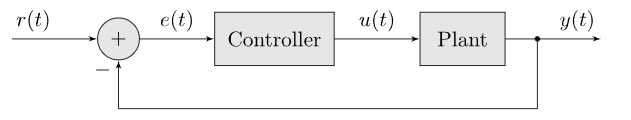
\includegraphics[width=0.7\linewidth]{figures/controller.png}
    \caption{Closed-Loop Error Feedback Controller}
    \label{fig:enter-label}
\end{figure}
where $r(t)$ is the desired value, $y(t)$ is the measured output, and $u(t)$ is the control input.
A PID controller stands for proportional, differential, and integral control. These are a set of numerical constants, or gains, that are multiplied to an error signal to compute a control input $u(t)$. 

The equations for a PID controller are as follows:

\begin{equation}
    e(t)=r(t)-y(t)
\end{equation}

\begin{equation}
u(t)=K_pe(t)+K_i\int_0^{t}e(\tau)d\tau+K_d\dot{e}(t)
\end{equation}

 where $K_p,  K_i$, and $K_d$ are the controller gains. Taking the Laplace domain of Equation 2.4 results in Equation 2.5.

\begin{equation}
    U(s)=(K_p+K_i\frac{1}{s}+K_ds)E(s)
\end{equation}

In short: the proportional control responds to instantaneous error, the integral control accumulate error to minimize steady-state error, and derivative control penalizes the rate of change of the error. Let us now look at a block diagram for the PID control system, shown in Figures 2.3 and 2.4.

\begin{figure}[h]
    \centering
    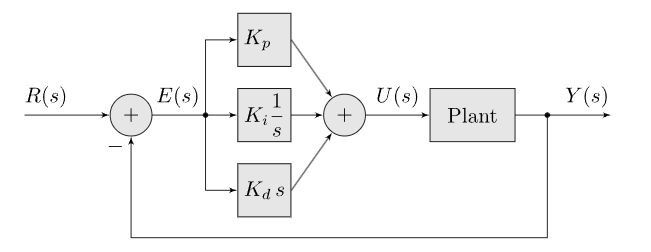
\includegraphics[width=0.8\linewidth]{figures/PID_freq.png}
    \caption{PID Control System (Time Domain)}
    \label{fig:enter-label}
\end{figure}

\begin{figure}[h]
    \centering
    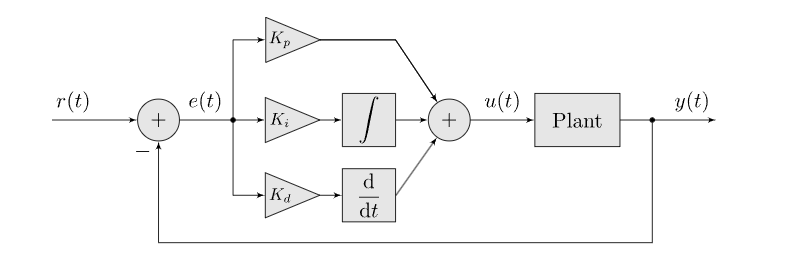
\includegraphics[width=0.8\linewidth]{figures/PID_time.png}
    \caption{PID Control System (Frequency Domain)}
    \label{fig:enter-label}
\end{figure}

The closed-loop transfer function can be calculated and analyzed to tune the gains. 

\begin{equation}
    G(s)=\frac{P(s)C(s)}{1+P(s)C(s)}
\end{equation}
where now $G(s)=\frac{Y(s)}{R(s)}$, $C(s)=\frac{U(s)}{E(s)}$, and $P(s)=\frac{Y(s)}{U(s)}$. Note that $P(s)$ is the previous $G(s)$ from before and now $G(s)$ represents the closed-loop transfer function (standard notation is confusing sometimes).
 To tune the gains, certain parameters can be looked at such as stability, rise time, settling time, and overshoot through eigenvalue analysis and time-domain simulations. 

Note that in reality, a numerical calculation of the error derivative requires a future measurement, so a filter always is put on the derivative gain to make the system 'causal'. Additionally, control systems are not continuous as they are implemented in computers and micro-controllers, which are inherently discrete systems. Therefore the PID control law needs to be discretized. Software libraries for designing PID controllers typically will do this process already, but it can be done manually if desired.

Tuning, filtering, and discretization of the control system is out of the scope of this document, as the focus is on system identification (for now).

\subsection{System Identification}
Recall that in the Laplace domain $s$ is a complex variable $s=\sigma+j\omega$. When performing system identification, we often only care about the frequency response of a system and set $\sigma=0$. In short, the focus is on the steady-state behavior, and the approximation $G(s)=G(j\omega)$ is made, and is true for LTI systems. Note that Elysium is a time-varying system, so this is an approximation we have to make.

Taking the Fourier transforms of the signals $u(t)$ and $y(t)$ results in their frequency domain counterparts, $U(j\omega)$ and $Y(j\omega$). The transfer function $G(j\omega)$ can be simply calculated through Equation 2.7. 

\begin{equation}
    G(j\omega)=\frac{Y(j\omega)}{U(j\omega)}
\end{equation}

However, this only works well for linear, noise-free systems. Using spectral analysis, the auto-power spectral density and the cross-power spectral density are calculated to get a better estimate of the function $G(j\omega)$.

\begin{equation}
    G(j\omega)=\frac{Y(j\omega)\cdot U^*(j\omega)}{U(j\omega)\cdot U^*(j\omega)}=\frac{Y(j\omega)}{U(j\omega)}
\end{equation}

This method reduces noise impacts and handles stochastic I/O better. An explanation on spectral analysis is out of the scope of this document. See Welch's Method for a similar but somewhat more robust system identification method using spectral analysis.

Using this method, we can take the FFT of $u(t)$ and $y(t)$ from test data and calculate the transfer function $G(j\omega) \approx G(s)$ to identify the plant $P(s)$ by curve-fitting a polynomial on $G(jw)$. With $P(s)$ approximated, it can be put into MATLAB/Simulink to design and tune the PID controller.

\subsection{System Identification Example}


In this example we will identify the spring-mass-damper system in Figure 2.1 and compare it to the analytical solution. This spring-mass-damper is represented with a State-Space model of Equation 2.1, and it's output is sampled at 32 Hz. Note that in this example, the output is $\ddot{x}(t)$ instead of $x(t)$.

\begin{lstlisting}[style=Matlab-editor, caption={\texttt{Defining The System}},frame=single, numbers=left]
%%%%%%%%%%%%%%%%%%%%%%%%%%%%%%%%%%%%%%%%%%%%%%%%%%%%%%%%%%%%%%%%%%%%%%%
%% Define the System (Spring Mass Damper, State-Space Representation) 

% Continuous Dynamics
k = 1;                          % spring constant
c = 0.01;                       % damping coefficient
A = [0  1; -k -c];              % continuous A matrix
B = [0; 1];                     % continuous B matrix
C = [-1 -c];                    % C matrix
D = 1;                          % D matrix

% Discretized Dynamics
fs = 32;                        % sampling frequency
dt = 1/fs;                      % samplinng time step
Ad = expm(A*dt);                % discrete A matrix
Bd = (Ad - eye(2))*A^-1*B;      % discrete B matrix

% Simulation Time
T0 = 0;                         % given initial time
Tf = 1024;                      % given final time (1024 samples)
T = T0:1/fs:(Tf - 1/fs);        % time values

% Frequencty Range (Nyquist Freq. = 1/2 Sampling Freq)
Np = length(T);
w = 0.5*fs*linspace(0,1,Np/2 + 1);  

\end{lstlisting}

\begin{lstlisting}[style=Matlab-editor, caption={\texttt{Analytical Transfer Function}},frame=single, numbers=left]
%%%%%%%%%%%%%%%%%%%%%%%%%%%%%%%%%%%%%%%%%%%%%%%%%%%%%%%%%%%%%%%%%%%%%%%
%% Analytical Transfer Function 

% Analytical Solution to get |G(jw)| vs w
s = 1i*(2*pi)*w;                    % s = jw
G = 1./(s.^2 + c*s + k);            % G(jw)

mag_analytical = 20*log10(abs(G));  % |G(jw)| in dB
\end{lstlisting}

 Note that from the Nyquist-Shannon sampling theorem, you can only obtain the frequency content of a signal up to half of it's sampling frequency when performing an FFT (due to aliasing). The next step is to simulate the sampled output data given a random control input.

\begin{lstlisting}[style=Matlab-editor, caption={\texttt{Simulating a Random Control Input}},frame=single, numbers=left]
%%%%%%%%%%%%%%%%%%%%%%%%%%%%%%%%%%%%%%%%%%%%%%%%%%%%%%%%%%%%%%%%%%%%%%%
%% Generate Sample Data

% Control Input
Ne = Np/4;
u = zeros(1,Np);
u(1:Ne)= randn(1,Ne).*hann(Ne).';   % u(t) = Random Force on Mass

% Simulate the System
x = [0; 0];
y = C*x + D*u(1);
for i = 2:length(T)
    x = Ad*x + Bd*u(i);
    y = [y (C*x + D*u(i))];         % y(t) = Acceleration of Mass
end
\end{lstlisting}

Using spectral Analysis, the transfer function can be identified with a polynomial curve fit.

\begin{lstlisting}[style=Matlab-editor, caption={\texttt{System Identification, Method 1}},frame=single, numbers=left]
%%%%%%%%%%%%%%%%%%%%%%%%%%%%%%%%%%%%%%%%%%%%%%%%%%%%%%%%%%%%%%%%%%%%%%%
%% Emperical G(jw) using u(t) and y(t) sample data

% Self-coded method to get |G(jw)| vs. w
U = fft(u, Np)/Np;                  % DFT of u(t) to get U(jw)
Y = fft(y, Np)/Np;                  % DFT of y(t) to get Y(jw)

YU = Y.*conj(U);                    % Cross-corellation function
UU = U.*conj(U);                    % Auto-corellation function
G1 = YU./UU;                        % Calculate G(jw)

mag_emperical_v1 = 20*log10(abs(G1));    % |G(jw)| DFTs 

% objective function
s = 1i*(2*pi)*w;
G = G(1:Np/2+1);
J = @(p) sum(1./(s.^2 + s.*p(1) + p(2)) - G).^2;

% perform optimization
p0 = [0.03, 1.02];         % initial guess for [c, k]
p_est = fminsearch(J, p0);
c_est = p_est(1);
k_est = p_est(2);

% estimated transfer function using fitted params
G_fit = 1 ./ (s.^2 + s*c_est + k_est);
mag_est_v1 = 20*log10(abs(G_fit));      % |G(jw)| identified
\end{lstlisting}

MATLAB has some functions that can be used from the System Identification toolbox instead. This toolbox uses its own spectral analysis and curve fitting method.
\begin{lstlisting}[style=Matlab-editor, caption={\texttt{System Identification, Method 2}},frame=single, numbers=left]
%%%%%%%%%%%%%%%%%%%%%%%%%%%%%%%%%%%%%%%%%%%%%%%%%%%%%%%%%%%%%%%%%%%%%%%
%% Identified G(jw) using u(t) and y(t) sample data

% MATLAB function to get |G(jw)| vs. w 
G2 = tfestimate(u,y,Np,[],[], fs);
mag_emperical_v2 = 20*log10(abs(G2));         % |G(jw)| using tfestimate()

% MATLAB function to get G(s) = 1/(s^2 + cs + k)
data = iddata(y', u', dt);
tf_est = tfest(data, 2);                       % G(s) using tfest()
[G_est, ~] = bode(tf_est, (2*pi)*w);           % G(jw) using tfest()

mag_est_v2 = 20*log10(squeeze(G_est));         % |G(jw)| using tfest()
\end{lstlisting}

Lastly, plots comparing the two system identification methods to the analytical solution can be made. Note that the natural frequency $\omega_n=\sqrt{\frac{k}{m}}$ is calculated to compare to the Bode plots of the transfer function.

\begin{lstlisting}[style=Matlab-editor, caption={\texttt{Plot the Results}},frame=single, numbers=left]
%%%%%%%%%%%%%%%%%%%%%%%%%%%%%%%%%%%%%%%%%%%%%%%%%%%%%%%%%%%%%%%%%%%%
%% Plot the Data

% plot the sampled control
figure; 
subplot(2,1,1);
stairs(T,u, 'k'); xlim([T0, Tf]);
ylabel("$u(t)$", Interpreter='latex');
title("Control \& Acceleration vs. Time", Interpreter="latex")

% plot the sampled acceleration
subplot(2,1,2);
stairs(T, y, 'k'); xlim([T0, Tf])
ylabel("$\ddot{x}(t)$", Interpreter='latex');
xlabel("$t$ (s)", Interpreter="latex")

% plot the DFT magnitude
figure(); 
plot(w,mag_analytical, 'k', 'LineWidth', 1.5, ...
    "DisplayName","Analytical G(s)"); hold on;
plot(w,mag_emperical_v1(1:Np/2+1), 'r-', ...
    "DisplayName","Emperical DFT - custom code" ); 
plot(w,mag_emperical_v2, 'b-', ...
    "DisplayName","Emperical DFT - tfestimate()"); 
plot(w,mag_est_v1, 'r--', ...
    "DisplayName","Identified G(s) - custom code" );
plot(w,mag_est_v2, 'b--', ...
    "DisplayName","Identified G(s) - tfest()"); 
ylim([-60 60]); 
xlim([w(1) 0.5]);
ylabel("$|G(j\omega)|$ (dB)", Interpreter="latex");
xlabel("$\omega$ (Hz)", Interpreter="latex")
grid on; 
title("$G(s)=\frac{1}{s^2+cs+k}$", Interpreter="latex")
legend();

% natural frequency
w_n = sqrt(k) / (2*pi);
disp(w_n)
\end{lstlisting}

The natural frequency of the system was calculated to be 0.1592 analytically. The system was very accurately identified using both methods, as shown in Figure 2.5.

\begin{figure}[h]
    \centering
    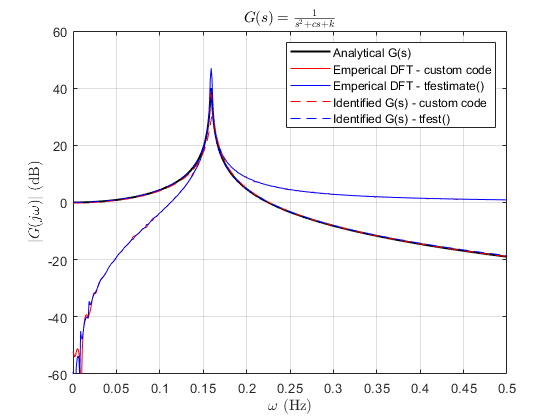
\includegraphics[width=1\linewidth]{figures/example_plots.png}
    \caption{System Identification Results}
    \label{fig:enter-label}
\end{figure}

\newpage

\section{Throttle to Thrust System Identification}

In the example from Section 2, it was explored how to identify a system based given data from a random input and the measured output. For Elysium, the same analysis can be performed, however, the input will not be random.

The purpose of the random input was to get a wide spectrum of frequency content of the input signal. I anticipate the throttle to be a generally low-frequency process, so I think we can get away with just varying a sinusoidal throttle input. I also think that we can just model both throttle valves as a single throttle valve, just opening and closing them the same amount.

I have spoken a lot with SRT on their throttle design (I told them to use this method as well), and this is what we came up with for a throttle input to look like for a test. 

\begin{figure}[h]
    \centering
    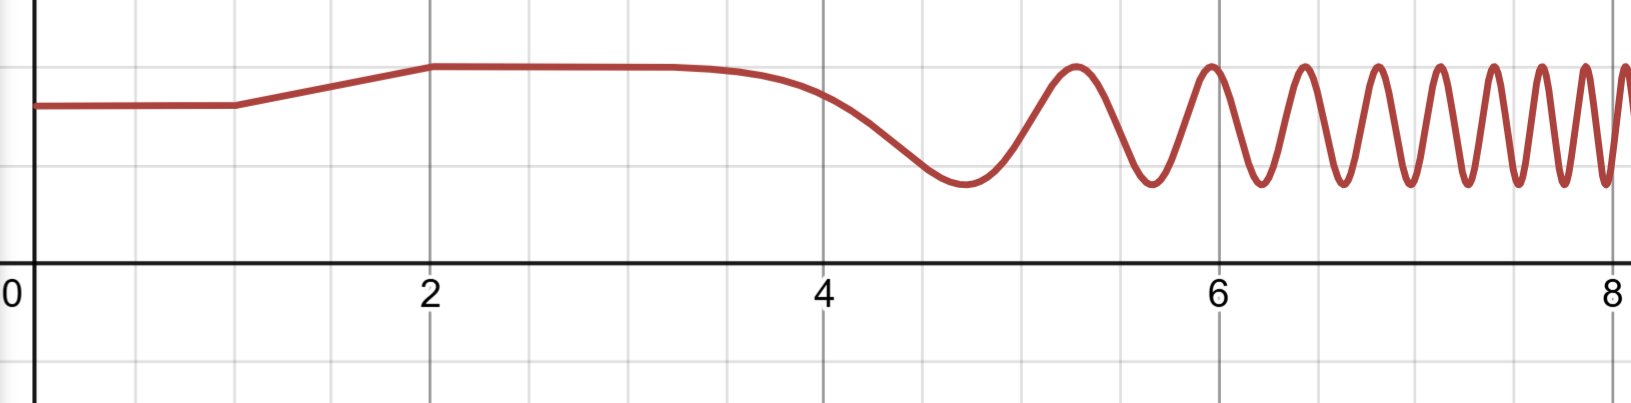
\includegraphics[width=1\linewidth]{figures/throttle_curve.png}
    \caption{Throttle Curve Example (\% throttle as a function of time)}
    \label{fig:enter-label}
\end{figure}

What this will do is get a mix of a step response and a sweep of increasing frequencies to get how the system responds at higher frequencies. This should get us a pretty good idea of how the system will respond to our throttle inputs from just one test. Aside from system identification, I don't anticipate to throttle at those higher frequencies during nominal operations. 

From Section 2.3, using \texttt{fft()} on the $u(t)$ data and $y(t)$ data (throttle \% and thrust), the magnitude of the transfer function can bee calculated with the following equation (Equation 2.8):

\begin{equation*}
    G(j\omega)=\frac{Y(j\omega)\cdot U^*(j\omega)}{U(j\omega)\cdot U^*(j\omega)}=\frac{Y(j\omega)}{U(j\omega)}
\end{equation*}

This equation can be implemented in MATLAB with \texttt{YU = Y.*conj(U)}, \texttt{UU = U.*conj(U)}, and \texttt{G = YU./UU}. Any method to curve fit $G(j\omega)$ to \texttt{G} can be used to get the transfer function.

\section{Throttle Controller Design}

Once the system is identified, the PID controller can be designed in MATLAB simulink. An example of how the control loop may look is as follows:

\begin{figure}[h]
    \centering
    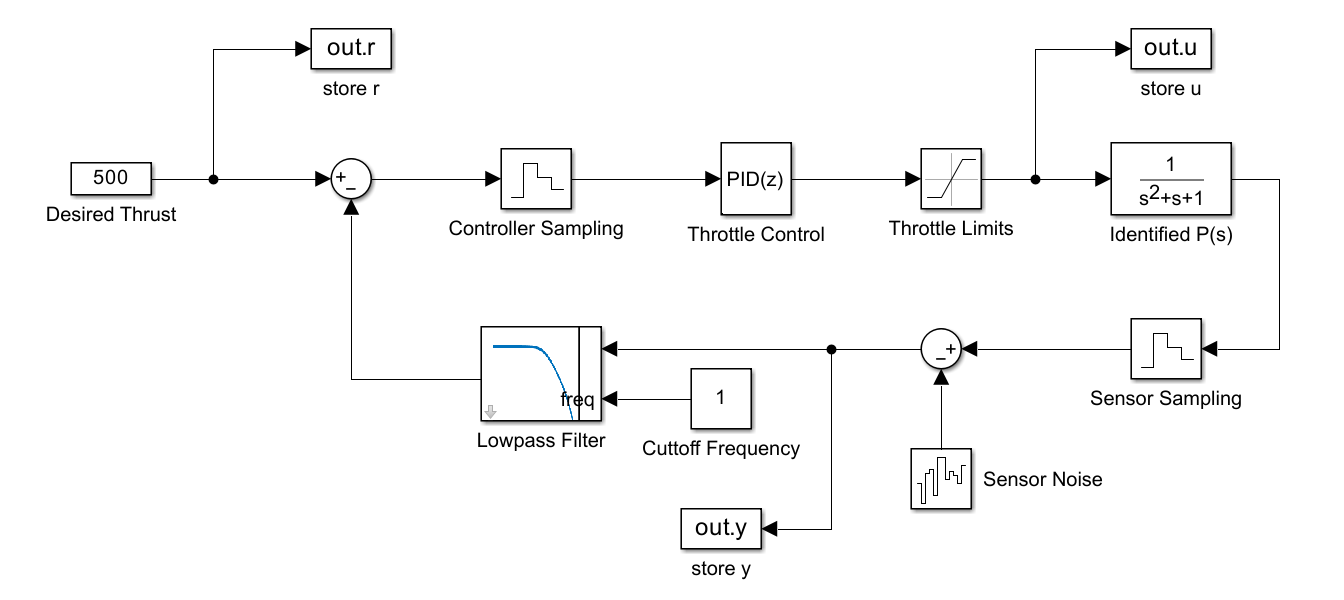
\includegraphics[width=1\linewidth]{figures/simulink_diagram.png}
    \caption{Simulink Diagram}
    \label{fig:enter-label}
\end{figure}

This uses a discrete-time PID controller with the continuous-time plant, just like how the real system will be. There are throttle limits in place, and a sensor has been modeled as well.

Some learning on how to operate simulink is necesarry, and learning on how to tune a PID controller is needed as well. These are out of the scope of this document (for now). Note that you may not even need a controller if the engine dynamics are steady and linear in thrust vs throttle \% . That would mean a simple $70\%$ throttle position = $70\%$ thrust.
\end{document}